%%%%%%%%%%%%%%%%%%%%%%%%%%%%%%%%%%%%%%%%%%%%%%%%%%%%%%%%%%%%%%%%%%%%%%
%%                     absolute inhibition
%%%%%%%%%%%%%%%%%%%%%%%%%%%%%%%%%%%%%%%%%%%%%%%%%%%%%%%%%%%%%%%%%%%%%%
\color{ForestGreen}

\subsubsection{Glyph: \glyph{Absolute inhibition}}\label{sec:absoluteInhibition}

An absolute inhibition precludes the existence of another relationship. A relationship modulated by an absolute inhibition can only exist when an absolute inhibition in false, whatever are the other influences this relationship is subjected to.

\begin{glyphDescription}
 \glyphSboTerm SBO:0000171 ! absolute inhibition.
 \glyphOrigin Any \glyph{interactor} (\sect{interactors}) or any \glyph{logical operator} (\sect{logic}).
 \glyphTarget Any \glyph{statement} (\sect{statements}) or \glyph{influence} (\sect{influences}).
 \glyphEndPoint The target extremity of a \glyph{absolute inhibition} carries a double bar perpendicular to the arc (to remind that it is an \glyph{inhibition}).
 \end{glyphDescription}

\begin{figure}[H]
  \centering
  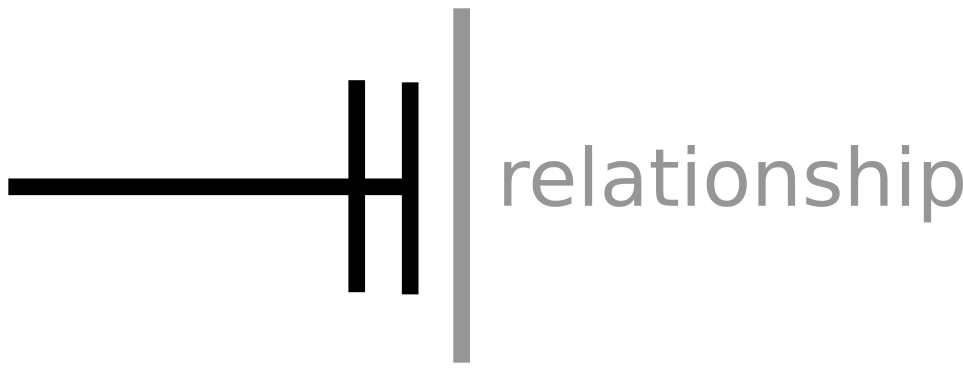
\includegraphics[scale = 0.3]{images/absoluteInhibition}
  \caption{The \PD glyph for \glyph{absoluteInhibition}.}
  \label{fig:absoluteInhibition}
\end{figure}

\begin{figure}[H]
  \centering
  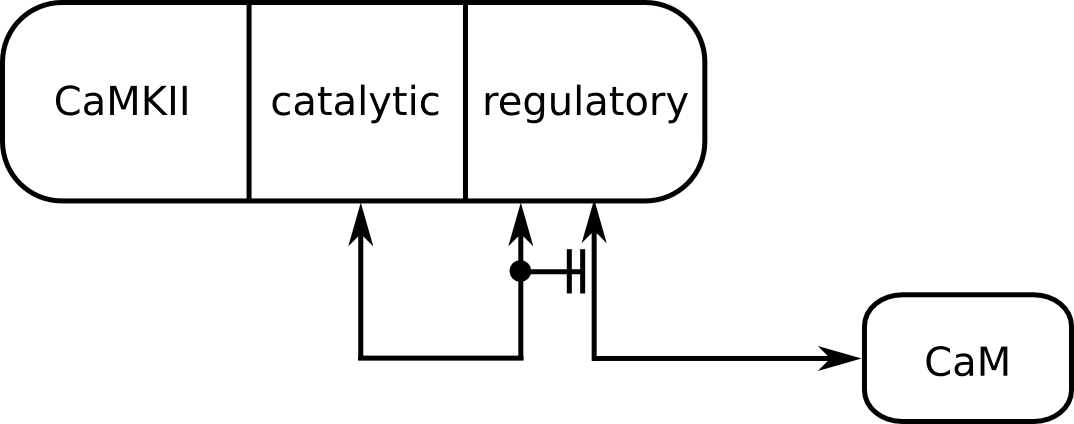
\includegraphics[scale = 0.5]{examples/ex-absoluteInhibition}
  \caption{This example shows how the interaction between catalytic and regulatory domains of CaMKII precludes the interaction of Calmodulin with CaMKII.}
  \label{fig:ex-absoluteInhibition}
\end{figure}

\normalcolor